\documentclass[10pt]{article}
\usepackage[a4paper,margin=1.3cm,top=1.0cm,bottom=1.0cm]{geometry}
\usepackage[T1]{fontenc}
\usepackage{lmodern}
\usepackage{microtype}
\usepackage{booktabs}
\usepackage{enumitem}
\usepackage{titlesec}
\usepackage{tikz}
\usetikzlibrary{arrows.meta,positioning}
\usepackage[hidelinks]{hyperref}

\titleformat{\section}{\normalfont\normalsize\bfseries}{\thesection}{0.6em}{}
\titlespacing*{\section}{0pt}{3pt}{0pt}
\titleformat{\subsection}{\normalfont\normalsize\bfseries}{\thesubsection}{0.6em}{}
\titlespacing*{\subsection}{0pt}{3pt}{1pt}
\setlist{itemsep=0pt,topsep=1pt,parsep=0pt,leftmargin=1.2em}
\setlength{\parindent}{0pt}
\setlength{\parskip}{2pt}
\pagestyle{empty}
\emergencystretch=1em

\newcommand{\cfg}[1]{\texttt{#1}}

\begin{document}

\begin{center}
  {\Large\bfseries The \cfg{ultra} preconfiguration of KaHIP}\\[3pt]
  {\normalsize Christian Schulz \quad$\cdot$\quad November 17, 2026}
\end{center}

\vspace{-2pt}
\textbf{Goal.} Spend the time v3.26 saved over v3.25 on better cuts: \cfg{ultra} starts from \cfg{strong}, keeps
its balance rule, stays within v3.25 \cfg{strong}'s time on every job, and should also make kaffpaE and KaBaPE better
at a fixed time limit. Every change is guarded by a field that only \cfg{ultra} sets.
\cfg{ultra} was developed with Agentic Algorithm Engineering (AAE)~[1], run with a focus on solution quality: each
change was stated as a hypothesis, implemented, measured on a fixed benchmark against a fixed quality gate, and kept
only if the cuts improved.

\begin{center}
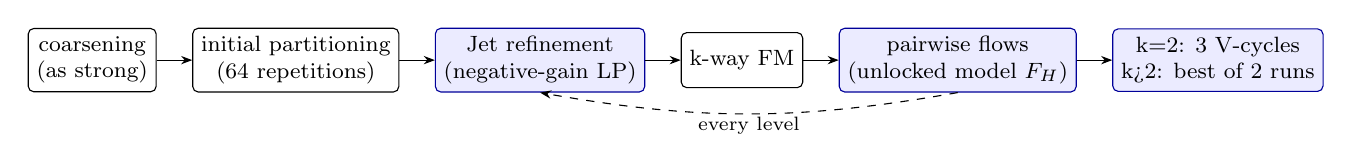
\begin{tikzpicture}[
  box/.style={draw,rounded corners=2pt,align=center,font=\footnotesize,minimum height=7mm,inner sep=3pt},
  new/.style={box,fill=blue!8,draw=blue!60!black},
  >={Stealth[length=4pt]}, node distance=4.5mm]
  \node[box] (c) {coarsening\\(as strong)};
  \node[box,right=of c] (ip) {initial partitioning\\(64 repetitions)};
  \node[new,right=of ip] (jet) {Jet refinement\\(negative-gain LP)};
  \node[box,right=of jet] (fm) {k-way FM};
  \node[new,right=of fm] (flow) {pairwise flows\\(unlocked model $F_H$)};
  \node[new,right=of flow] (rep) {k=2: 3 V-cycles\\k>2: best of 2 runs};
  \draw[->] (c) -- (ip); \draw[->] (ip) -- (jet); \draw[->] (jet) -- (fm); \draw[->] (fm) -- (flow);
  \draw[->] (flow) -- (rep);
  \draw[->,dashed] (flow.south) to[bend left=10] node[below=1pt,font=\scriptsize,inner sep=0pt,fill=white]{every level} (jet.south);
\end{tikzpicture}
\end{center}
\vspace{-6pt}

\section{ultra kaffpa (sequential multilevel)}
\begin{itemize}
  \item \textbf{Jet refinement}~[2] runs on every level before the k-way FM
  (field \cfg{jet\_refinement}, code in \cfg{jet\_refinement.cpp}). Jet is synchronous label
  propagation that also accepts bounded negative-gain moves, so FM starts outside its own local optimum.
  \begin{itemize}
    \item \emph{Candidates.} Every unlocked boundary node $v$ of a block $A$ picks the adjacent block $B$ it is most
    strongly connected to (ties: the lighter block). With gain $g(v)=\omega(v,B)-\omega(v,A)$, $v$ becomes a
    candidate if $g(v)\ge 0$ or the loss $-g(v)$ is below $c\cdot\omega(v,A)$, with $c=0.25$ for unit
    node weights and $c=0.75$ otherwise.
    \item \emph{Afterburner.} Each candidate recomputes its gain as if every candidate of higher rank (larger
    gain, ties by node ID) had already moved to its target. Only candidates whose recomputed gain is $\ge 0$
    move, all at once; moved nodes are locked for the next iteration.
    \item \emph{Rebalancing.} If the heaviest block exceeds the bound, the iteration rebalances instead: in every
    overloaded block, nodes are sorted by loss per node weight and moved, cheapest first, until the block fits.
    Boundary nodes go to their best-connected block with room; interior nodes go to the lightest block.
  \end{itemize}
  Jet keeps the partition with the smallest cut whose heaviest block is not heavier than the bound (or the input,
  if that was heavier). It stops after 12 iterations without a cut below $0.999$ times the best (at most 100
  iterations); only nodes next to a move are evaluated again.
  \item \textbf{Unlocked flow model $F_H$}~[3] (field \cfg{flow\_unlocked\_model}, code in
  \cfg{cut\_flow\_problem\_solver.cpp}) in the pairwise flow refinement. For each pair of adjacent blocks $(A,B)$, KaHIP grows a region around
  their boundary by BFS in both blocks, sized with the flow region factor $\alpha=8$ (as in \cfg{strong}) so
  that every minimum cut gives a balanced partition, and solves a max-flow problem on it. In the original model
  the outer border of the region is tied to the source (in $A$) or the sink (in $B$) with infinite capacity, so
  these nodes can never change sides. In $F_H$, each region node $v$ gets a source edge with the weight of its edges
  to $A$ outside the region and a sink edge with the weight of its edges to $B$ outside the region; edges to third
  blocks are left out, since they are cut on either side. The value of an $s$-$t$ cut is then exactly the
  $A$--$B$ cut of the partition it induces, and the same region offers a larger space of cuts. Without any source or sink
  edge, the original model is used. As in \cfg{strong}, the most balanced minimum cut is taken. A long-standing
  flow bug (no flow network could be built, but the old cut was stored anyway) is fixed in v3.28 for all configurations.
  \item \textbf{More global work:} for $k=2$, 3 V-cycles instead of 2; for $k>2$, the best of 2 independent runs.
  Inside kaffpaE each operator makes a single run.
\end{itemize}

\section{ultra kaffpaE / KaBaPE (memetic, MPI)}
kaffpaE and KaBaPE (kaffpaE at $\varepsilon=0$) run the \cfg{ultra} kaffpa above in every operator (initial
population, combine, mutation), one run each. Two changes apply to the evolutionary algorithm itself:
\begin{itemize}
  \item \textbf{Balanced individuals first} (\cfg{mh\_penalty\_for\_imbalance}). An individual that exceeds the balance
  bound gets the fitness ``total edge weight $+\,1+$ overload'', so it ranks behind every balanced individual in
  selection, exchange and the final choice. If the final partition still exceeds the bound, a negative-cycle
  rebalance moves nodes until every block fits.
  \item \textbf{Keep the input partition} (\cfg{mh\_keep\_input}). If kaffpaE is started with
  \cfg{-{}-input\_partition}, that partition enters the population unchanged, so the result is never worse than the
  input; a second run thus restarts from the best partition found so far.
\end{itemize}

\section{Usage and compatibility}
\cfg{-{}-preconfiguration=ultra} for kaffpa, kaffpaE and KaBaPE; mode \cfg{ULTRA} (= 6) in the C/C++ interface and
\cfg{kahip.ULTRA} in Python; settings in \cfg{configuration::ultra} (\cfg{app/configuration.h}). All new code is
behind fields that only \cfg{ultra} sets, so every other preconfiguration gives the partitions of v3.26 (checked on
2907 runs and all 3469 command-line paths), except rare changes in \cfg{strong} and \cfg{strongsocial} from the flow fix.

\section{Key results}
\begin{tabular}{@{}ll@{}}
\toprule
kaffpa cuts & vs v3.26 \cfg{strong} (eps 3\%, 73 jobs): Q 0.9777 (tuning and held-out graphs), 0.9729 (new seeds)\\
kaffpa time & 2.0$\times$ v3.26 \cfg{strong}; below v3.25 \cfg{strong} on every job (geomean 0.64 of it)\\
kaffpaE, KaBaPE & same time limit, vs \cfg{strong} inside: QE 0.991--0.995 (kaffpaE), 0.984--0.987 (KaBaPE)\\
\bottomrule
\end{tabular}


\vspace{2pt}
{\footnotesize\textbf{References.}
[1]~D.~A. Bader, A.~Chhabra, E.~Gro{\ss}mann, M.~Henzinger, A.~Noe, C.~Schulz. Agentic algorithm engineering: Improving shared-memory exact minimum cuts. \emph{CoRR} abs/2609.07204, 2026; code: \href{https://github.com/CHSZLab/AgenticAlgorithmEngineering}{github.com/CHSZLab/AgenticAlgorithmEngineering}.
[2]~M.~S. Gilbert, K.~Madduri, E.~G. Boman, S.~Rajamanickam. Jet: Multilevel graph partitioning on graphics processing units. \emph{SIAM J. Sci. Comput.} 46(5):B700--B724, 2024.
[3]~T.~Heuer, P.~Sanders, S.~Schlag. Network flow-based refinement for multilevel hypergraph partitioning. \emph{ACM J. Exp. Algorithmics} 24(1):2.3:1--2.3:36, 2019.\par}

\end{document}
